\documentclass{ctexart}

\usepackage{amsmath}
\usepackage{amssymb}
\usepackage{amsfonts}
\usepackage{mathabx}
\usepackage{listings}
\usepackage{tikz}
\usetikzlibrary{automata,positioning}

\usepackage{color}

\definecolor{mygreen}{rgb}{0,0.6,0}
\definecolor{mygray}{rgb}{0.5,0.5,0.5}
\definecolor{mymauve}{rgb}{0.58,0,0.82}

\lstset{ %
	backgroundcolor=\color{white},   % choose the background color; you must add \usepackage{color} or \usepackage{xcolor}
	basicstyle=\footnotesize,        % the size of the fonts that are used for the code
	breakatwhitespace=false,         % sets if automatic breaks should only happen at whitespace
	breaklines=true,                 % sets automatic line breaking
	captionpos=b,                    % sets the caption-position to bottom
	commentstyle=\color{mygreen},    % comment style
	deletekeywords={...},            % if you want to delete keywords from the given language
	escapeinside={\%*}{*)},          % if you want to add LaTeX within your code
	extendedchars=true,              % lets you use non-ASCII characters; for 8-bits encodings only, does not work with UTF-8
	frame=single,	                   % adds a frame around the code
	keepspaces=true,                 % keeps spaces in text, useful for keeping indentation of code (possibly needs columns=flexible)
	keywordstyle=\color{blue},       % keyword style
	language=Octave,                 % the language of the code
	otherkeywords={*,...},           % if you want to add more keywords to the set
	numbers=left,                    % where to put the line-numbers; possible values are (none, left, right)
	numbersep=5pt,                   % how far the line-numbers are from the code
	numberstyle=\tiny\color{mygray}, % the style that is used for the line-numbers
	rulecolor=\color{black},         % if not set, the frame-color may be changed on line-breaks within not-black text (e.g. comments (green here))
	showspaces=false,                % show spaces everywhere adding particular underscores; it overrides 'showstringspaces'
	showstringspaces=false,          % underline spaces within strings only
	showtabs=false,                  % show tabs within strings adding particular underscores
	stepnumber=1,                    % the step between two line-numbers. If it's 1, each line will be numbered
	stringstyle=\color{mymauve},     % string literal style
	tabsize=2,	                   % sets default tabsize to 2 spaces
	title=\lstname                   % show the filename of files included with \lstinputlisting; also try caption instead of title
}

\lstdefinestyle{customc}{
	belowcaptionskip=1\baselineskip,
	breaklines=true,
	frame=L,
	xleftmargin=\parindent,
	language=C,
	showstringspaces=false,
	basicstyle=\footnotesize\ttfamily,
	keywordstyle=\bfseries\color{green!40!black},
	commentstyle=\itshape\color{purple!40!black},
	identifierstyle=\color{blue},
	stringstyle=\color{orange},
}

\lstdefinestyle{customasm}{
	belowcaptionskip=1\baselineskip,
	frame=L,
	xleftmargin=\parindent,
	language=[x86masm]Assembler,
	basicstyle=\footnotesize\ttfamily,
	commentstyle=\itshape\color{purple!40!black},
}

\lstset{escapechar=@,style=customc}

\begin{document}

%\begin{tikzpicture}[shorten >=1pt,node distance=2cm,on grid,auto] 
%\node[state,initial] (q_1) {$q_1$};
%\node[state] (q_2) [right=of q_1] {$q_2$};

%\path[->]
%(q_1) edge node {$0:R$} (q_2)
%edge [loop above] node {$1:R$} ()
%edge node [right] {e} +(0,-1);
%;
%\end{tikzpicture}

\section*{}

\textbf{5.6} Write an abacus-machine flow chart for computing the quotient function quo of the preceding problem.

Solution:

$x$ and $y$ are stored in register $x$ and $y$, the result (quotinent) is stored in register $q$.

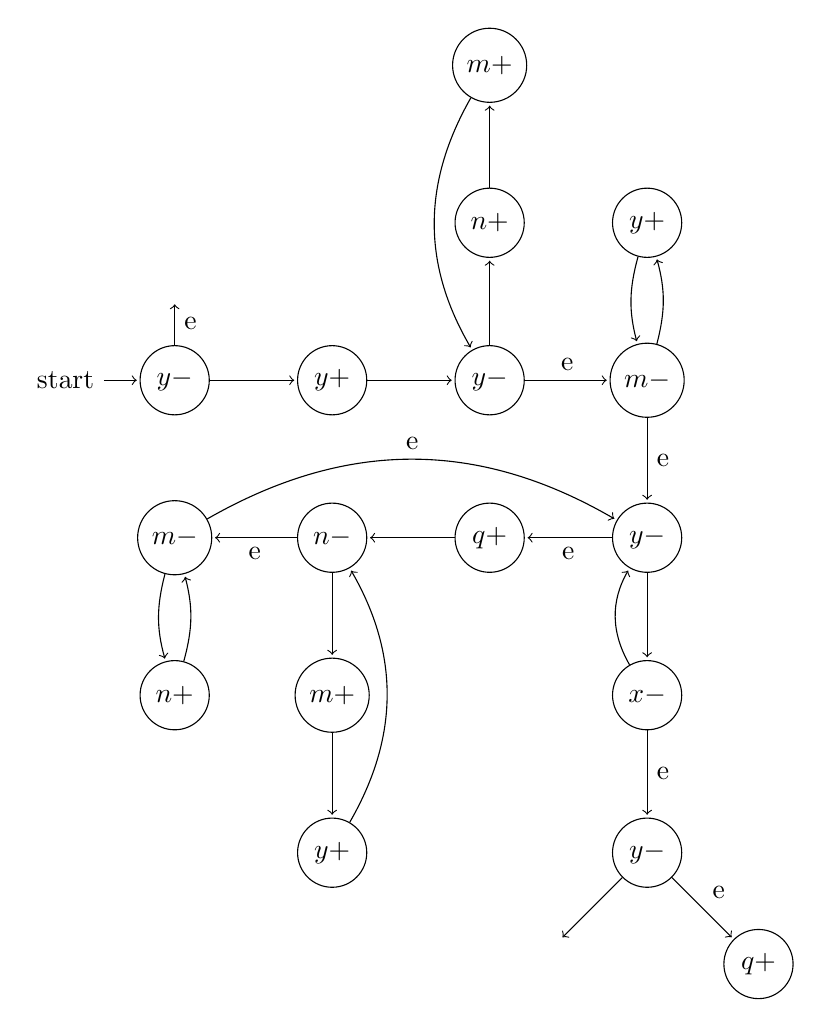
\begin{tikzpicture}[shorten >=1pt,node distance=2cm,on grid,auto] 
\node[state,initial] (q_1) {$y-$};
\node[state] (q_2) [right=of q_1] {$y+$};

\node[state] (q_3) [right=of q_2] {$y-$};
\node[state] (q_4) [above=of q_3] {$n+$};
\node[state] (q_5) [above=of q_4] {$m+$};
\node[state] (q_6) [right=of q_3] {$m-$};
\node[state] (q_7) [above=of q_6] {$y+$};

% subtract y
\node[state] (q_8) [below=of q_6] {$y-$};
\node[state] (q_9) [below=of q_8] {$x-$};
\node[state] (q_10) [left=of q_8] {$q+$};

\node[state] (q_11) [below=of q_9] {$y-$};
\node[state] (q_12) [below right=of q_11] {$q+$};

% restore y
\node[state] (q_13) [below=of q_2] {$n-$};
\node[state] (q_14) [below=of q_13] {$m+$};
\node[state] (q_15) [below=of q_14] {$y+$};
\node[state] (q_16) [left=of q_13] {$m-$};
\node[state] (q_17) [below=of q_16] {$n+$};

\path[->]
(q_1) edge node {} (q_2)
edge node [right] {e} +(0,1)
(q_2) edge node {} (q_3)

(q_3) edge node {e} (q_6)
edge node {} (q_4)
(q_4) edge node {} (q_5)
(q_5) edge [bend right=30] node {} (q_3)
(q_6) edge [bend right=15] node {} (q_7)
(q_7) edge [bend right=15] node {} (q_6)

%subtract y
(q_6) edge node {e} (q_8)
(q_8) edge node {} (q_9)
(q_8) edge node {e} (q_10)
(q_9) edge [bend left=30] node {} (q_8)
edge node {e} (q_11)
(q_11) edge node {e} (q_12)
edge node [right] {} +(-1.1,-1.1)

% restore y
(q_10) edge node {} (q_13)
(q_13) edge node {} (q_14)
(q_14) edge node {} (q_15)
(q_15) edge [bend right=30] node {} (q_13)
(q_13) edge node {e} (q_16)
(q_16) edge [bend right=15] node {} (q_17)
(q_17) edge [bend right=15] node {} (q_16)
(q_16) edge [bend left=30] node {e} (q_8)
;
\end{tikzpicture}

\section*{}

\textbf{6.6} An alternative coding of pairs of numbers by numbers was considered in
Example 1.2, based on the fact that every natural number n can be written
in one and only one way as 1 less than a power of 2 times an odd number,
$n = 2^{k(n)} (2l(n) \dotdiv 1) \dotdiv 1$. Show that the functions k and l are primitive recursive.

Solution:

If $n$ is even ($n + 1$ is odd), then $k(n) = 0$, $l(n) = \frac{n + 2}{2}$, obviously they are primitive recursive.

If $n$ is odd ($n+1$ is even), let $l(n) = \frac{n + 1}{2^{k(n) + 1}} + \frac 1 2$. $l(n)$ is primitive recursive if $k(n)$
is primitive recursive. Let $k(n) = \mathrm{lo}(n + 1)$, and $\mathrm{lo}(n)$ is primitive recursive, so be $k(n)$.

Define function
$$
odd(x') = \begin{cases}
0 & x' = 0 \\
1 - odd(x) & x' \ne 0
\end{cases}
$$
which is primitive recursive. Finally, we have
$$
k(n) = \begin{cases}
\mathrm{lo}(n + 1) & odd(n) = 1 \\
0 & odd(n) = 0
\end{cases}
$$
$$
l(n) = \begin{cases}
\frac{n + 1}{2^{k(n)+1}} + \frac 1 2 & odd(n) = 1 \\
\frac{n + 2}{2} & odd(n) = 0
\end{cases}
$$

\section*{}

\textbf{6.8} Given a reasonable way of coding recursive functions by natural numbers, let
d(x) = 1 if the one-place recursive function with code number x is defined and
has value 0 for argument x, and d(x) = 0 otherwise. Show that this function is
not recursive.

Solution:

Suppose function $c: f \to N$. Assuming $d(x)$ is recursive, let $c_d = c(d)$. $d(c_d) = 1$ if
$f_{c_d}(c_d) = d(c_d) = 0$, $d(c_d) = 0$ if $f_{c_d}(c_d) = d(c_d) \ne 0$. It's a contradition,
thus, $d(x)$ is not recursive.

\section*{}

\textbf{7.3} For natural numbers, write u | v to mean that u divides v without remainder,
that is, there is a w such that u · w = v. [Thus u | 0 holds for all u, but 0 | v
holds only for v = 0.] We say z is the greatest common divisor of x and y, and
write z = gcd(x, y), if z | x and z | y and whenever w | x and w | y, then w ≤ z
[except that, by convention, we let gcd(0, 0) = 0]. We say z is the least common
multiple of x and y, and write z = lcm(x, y), if x | z and y | z and whenever
x |w and y |w, then z ≤ w. Show that the functions gcd and lcm are primitive
recursive.

Solution:

$lcm(x, y) = \frac{x \times y}{gcd(x, y)}$, $lcm(x, y)$ is primitive recursive iff
$gcd(x, y)$ is primitive recursive.

Define $gcd(x, y) = h(x, y, x)$, where
$$
h(x, y, w') = \begin{cases}
0 & w' = 0 \\
w' & w' \ne 0, w' | x, w' | y \\
h(x, y, w) & \mathrm{otherwise}
\end{cases}
$$
Obviously $u | v = \overline{sg}(v \bmod u)$ is primitive recursive,
and its composition $h(x, y, w)$ is primitive recursive, too.

\section*{}

\textbf{7.6} Let f be a (primitive) recursive total function, and let A be the set of all n such
that the value f (n) is ‘new’ in the sense of being different from f (m) for all
m < n. Show that A is (primitive) recursive.

Solution:

Let $a(n)$ denotes the characteristic function of $A$
$$
a(n) = \forall_{m < n} f(m) \ne f(n)
$$
(primitive) Recursive relations are closed under bounded universal quantification, thus $A$ is
(primitive) recursive.

\section*{}

\textbf{7.11} Show that the substitution function of Example 7.22 is primitive recursive.

Solution:

Function $sub(s, c, d)$ can be expanded into
$$
sub(s, c, d) = \prod_{i=1}^{k} \left[
	\left(ent(s, i) = c \right) \times \pi(i)^d
	+
	\left(ent(s, i) \ne c \right) \times \pi(i)^{ent(s, i)}
	\right]
$$
Since all functions used in this formula are primitive functions, so be $sub(s, c, d)$.

\end{document}